% File : rev_literatura.tex


\chapter{Comparações}
%%%%%%%%%%%%%%%%%%%%%%%%%%%%%%%%%%%%%%%%%%%%%%%%%%%%%%%%%%%%%%%%%%%%%%%%%%%%%%%%%%%%%%%%%%%%%%%%%%%%%%%%%%%
%%%%%%%%%%%%%%%%%%%%%%%%%%%%%%%%%%%% AFAZERES_DOM %%%%%%%%%%%%%%%%%%%%%%%%%%%%%%%%%%%%%%%%%%%%%%%%%%%%%%%%%
%%%%%%%%%%%%%%%%%%%%%%%%%%%%%%%%%%%%%%%%%%%%%%%%%%%%%%%%%%%%%%%%%%%%%%%%%%%%%%%%%%%%%%%%%%%%%%%%%%%%%%%%%%%
\section{Tempo em afazeres domésticos}
O tempo gasto com afazeres domésticos pode privar o aluno de exercer o estudo
do ensino básico. Foram feitas análises sociais com base nas diferenças entre os 
períodos de tempo gastos diariamente nestas atividades.

%%%%% Gráfico de Sexo por afazeres_domesticos
\begin{figure}[h]
    \label{sexo_afazeres}
    \caption{Proporção dos sexos por período de tempo em afazeres domésticos por parte
    dos alunos.\label{sexo_afazeres}} % Pra fazer ref, tem q estar no caption
    \begin{center}
        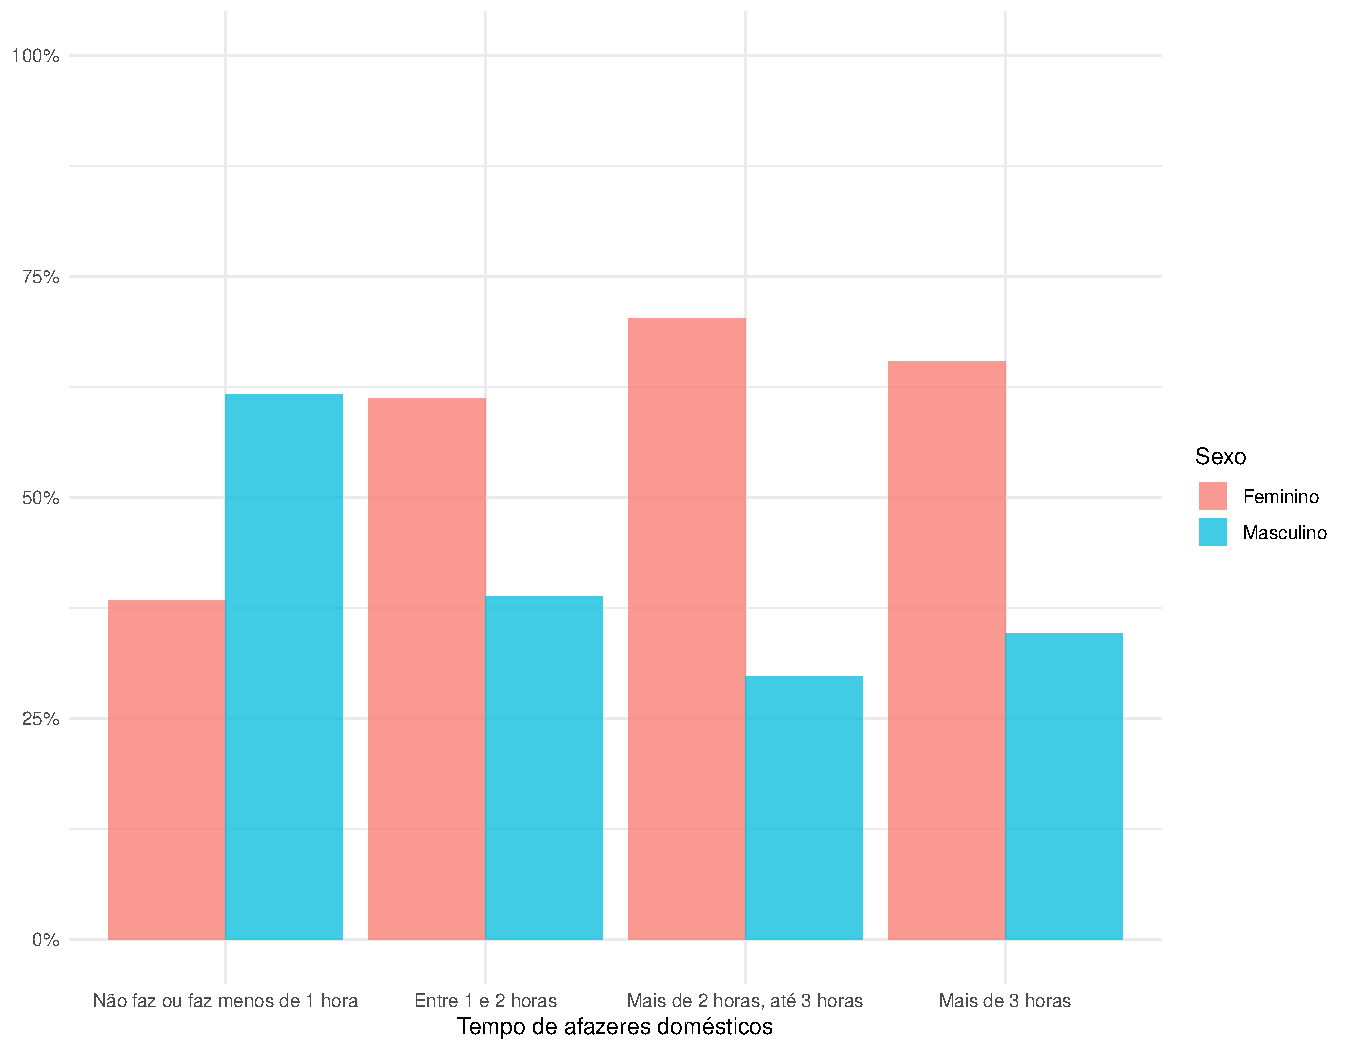
\includegraphics[width=16cm]{img/sexo_afazeres.pdf}
    \end{center}
    \fonte{Amostra de 5.271 alunos do 9\textsuperscript{o} ano do SAEB 2017.}
    \nota{Amostra retirada de uma amostragem aleatórias simples.}
\end{figure}

A \autoref{sexo_afazeres} apresenta como se distribuem estes períodos em relação ao sexo
do aluno, no qual estudantes do sexo feminino tendem a gastar mais tempo com atividades
domésticas. O único período em que o sexo feminino teve
menos representatividade foi a  categoria que menos tempo diário é gasto com atividades domésticas,
“Não faz ou faz menos de 1 hora”.

Para os períodos em que pelo menos uma hora por dia é gasta, o sexo feminino
representa no mínimo 60\% de todos os indivíduos, o que pode indicar que a proporção 
de estudantes do sexo masculino possui mais disponibilidade de tempo em casa para estudos.

%%%%% Gráfico de Escolaridade da mãe por afazeres_domesticos
\begin{figure}[h]
    \caption{Proporção total do nível de escolaridade da mãe
    com base nos períodos de tempo de afazeres domésticos por parte dos alunos.\label{esc_mae_afazeres}}
    \begin{center}
        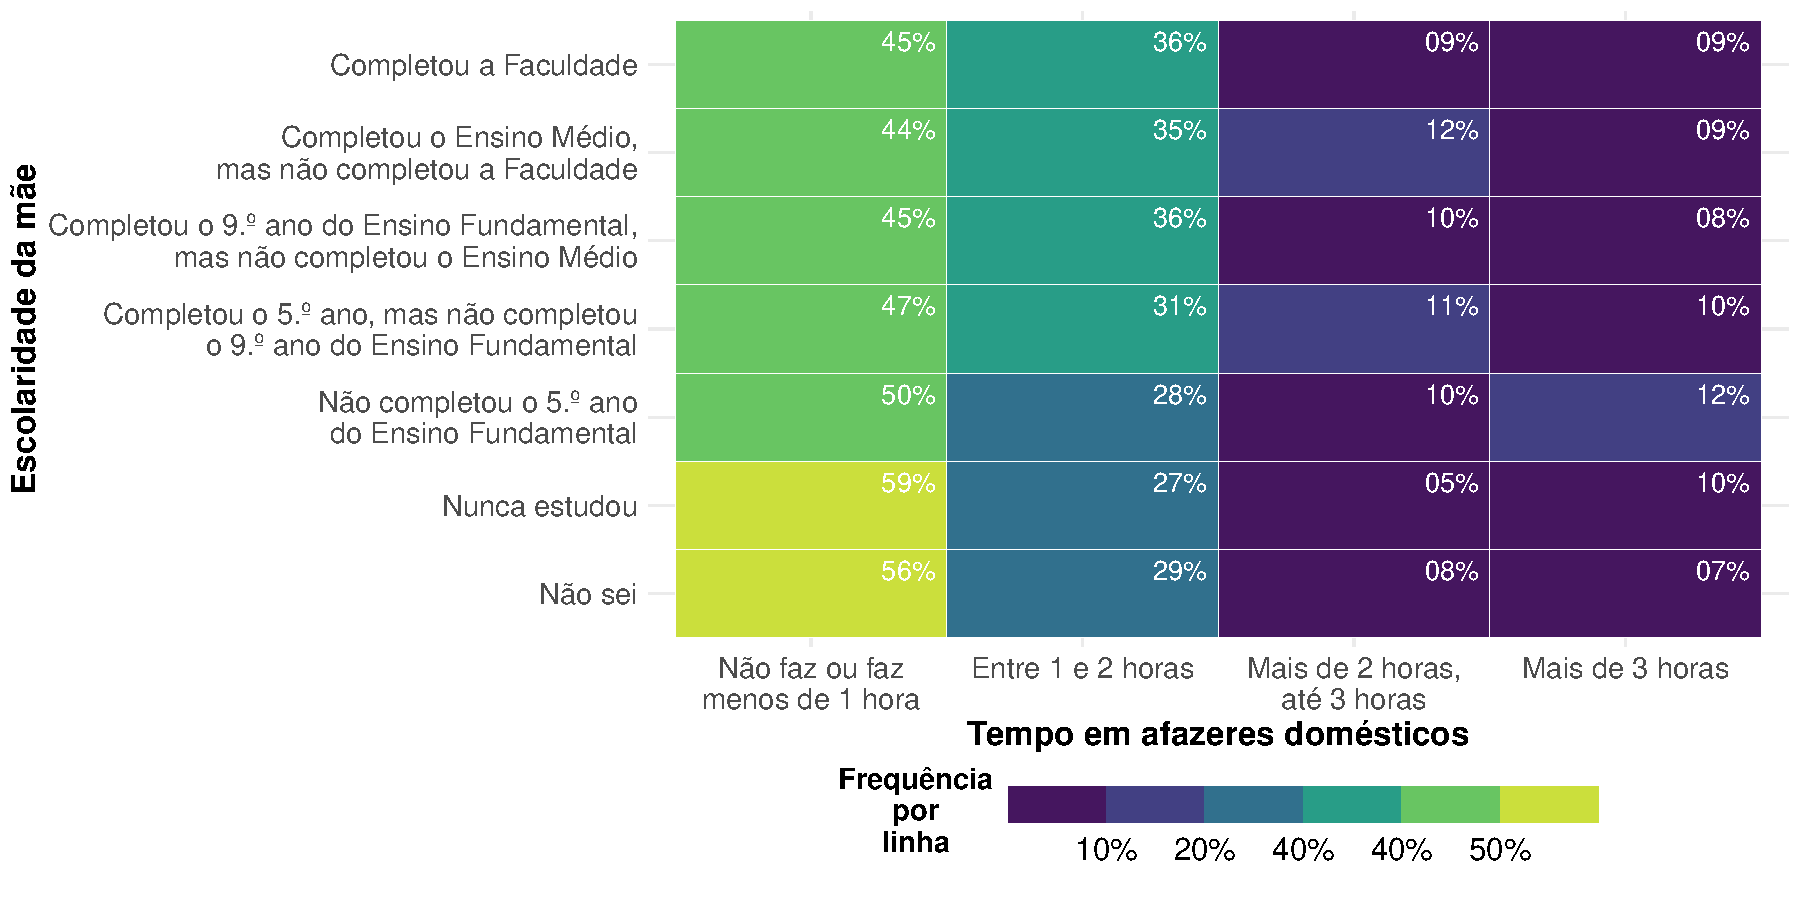
\includegraphics[width=16cm]{img/esc_mae_afazeres.pdf}
    \end{center}
    \fonte{Amostra de 5.271 alunos do 9\textsuperscript{o} ano do SAEB 2017.}
    \nota{Amostra retirada de uma amostragem aleatórias simples.}
\end{figure}

Outras observações sobre tempo gasto podem ser feitas ao observar a \autoref{esc_mae_afazeres},
que mostra o tempo gasto pelos alunos com atividades domésticas pra cada nível de escolaridade da mãe.
Ao analisar, a proporção de alunos que exercem estas atividade, sobre o total de alunos para cada nível
desta escolaridade, apresenta pelo menos 70\% localizado entre o período de tempo que 
não fazem ou fazem até 2 horas.
%%%%%%%%%%%%%%%%%%%%%%% Tabelas %%%%%%%%%%%%%%%%%%%%%%%%%%%%%%%%%%%%%%%%%%%%%%%%%%%%%%%%%%%%%%%%%

Os testes estatísticos, que avaliam a hipótese de igualdade das distribuições, com base nesses afazeres (\autoref{tab:af_test}) e com a
confiança de 95\%, a variável sexo obteve evidências significativas para afirmar que o tempo
médio não é igual entre os sexos, no qual o sexo feminino possui
proporções superiores em períodos de tempo maiores nestas atividades.

Ao testar a variável raça/cor dos alunos sob a mesma hipótese, não foram obtidas evidências significativas,
apontando que não há indícios de diferenças, em média, entre as raças/cores, no tempo gasto
nestes afazeres, assim como para a variável sobre a escolaridade da mãe com estes afazeres.



%%%%% Tabela dos testes paras relações com afazeres domesticos

\begin{table}[htb]
    \caption{Testes de igualdade na variabilidade sobre as relações 
            com o tempo de afazeres domésticos por parte dos alunos.\label{tab:af_test}}
        \centering
        \begin{tabular}{cccc}
        \toprule
        Teste & $H_0$& P-valor & Decisão de $H_0$ (95\%)\\
        \midrule \midrule
        K & $\mu_{Raça/Cor}$ iguais & 0.369 & Aceita\\
        K & $\mu_{Esc(mãe)}$ iguais & Aprox. 0 & Rejeita\\
        W & $\mu_M = \mu_F$ iguais & Aprox. 0 & Rejeita\\
        \bottomrule
        \end{tabular}
        \fonte{Amostra de 5.271 alunos do 9\textsuperscript{o} ano do SAEB 2017.}
        \nota{Amostra retirada de uma amostragem aleatória simples.}
        \nota[Anotações]{Os subíndices M e F referem-se, respectivamente, aos sexos Masculino e Feminino
        dos alunos. Esc (mãe) diz respeito à escolaridade da mãe destes. O Aprox. 0 refere-se a um número
        muito pequeno considerado por este estudo aproximadamente zero.}
\end{table}



%%%%% Tabela de comparação da escolaridade da mãe com afazeres domesticos
O teste realizado com base na escolaridade da mãe sobre o tempo em afazeres domésticos, obteve evidências significativas sobre a
existência de diferença no tempo gasto com afazeres domésticos. Ao efetuar testes pareados para cada 
nível escolar da mãe com a confiança de 95\% (\autoref{tab:esc_mae_afzr}) sobre essa mesma hipótese de igualdade, a proporção de alunos que gastam tempo nestes
afazeres, obteve diferenças nas distribuições apenas para aqueles que responderam não saber a escolaridade mãe com
os outros níveis desta escolaridade, exceto para aqueles que a mãe nunca estudou obteve igualdade.  
\clearpage

\begin{table}[htb]
    \centering
\caption{Comparações dois a dois entre as ordens das posições sobre os tempos de afazeres domésticos
com base na escolaridade das mães dos alunos\label{tab:esc_mae_afzr}}
    \begin{tabular}{lcc}
    \toprule
    Comparações & P-valor & Evidência (RA 95\%)\\
    \midrule \midrule
    Não sabe = Nunca estudou & 1.0000 & Iguais\\
    Não sabe = Incompleto 5.\textsuperscript{o} ano do EF  & 0.0078 & Desiguais\\
    Não sabe = Completou 5.\textsuperscript{o} ano do EF  & 0.0005 & Desiguais\\
    Não sabe = Completou 9.\textsuperscript{o} ano do EF  & 0.0001 & Desiguais\\
    Não sabe = Completou EM & Aprox. 0 & Desiguais\\
    Não sabe = Completou Faculdade & 0.0011 & Desiguais\\
    
    Nunca estudou = Incompleto 5.\textsuperscript{o} ano do EF  & 1.0000 & Iguais\\
    Nunca estudou = Completou 5.\textsuperscript{o} ano do EF  & 0.5598 & Iguais\\
    Nunca estudou = Completou 9.\textsuperscript{o} ano do EF  & 0.4165 & Iguais\\
    Nunca estudou = Completou EM & 0.1114 & Iguais\\
    Nunca estudou = Completou Faculdade & 0.4707 & Iguais\\
    
    Incompleto 5.\textsuperscript{o} ano do EF = Completou 5.\textsuperscript{o} ano do EF  & 1.0000 & Iguais\\
    Incompleto 5.\textsuperscript{o} ano do EF = Completou 9.\textsuperscript{o} ano do EF  & 1.0000 & Iguais\\
    Incompleto 5.\textsuperscript{o} ano do EF = Completou EM & 1.0000 & Iguais\\
    Incompleto 5.\textsuperscript{o} ano do EF = Completou Faculdade & 1.0000 & Iguais\\
    
    Completo 5.\textsuperscript{o} ano do EF = Completou 9.\textsuperscript{o} ano do EF  & 1.0000 & Iguais\\
    Completo 5.\textsuperscript{o} ano do EF = Completou EM & 1.0000 & Iguais\\
    Completo 5.\textsuperscript{o} ano do EF = Completou Faculdade & 1.0000 & Iguais\\
    
    Completo 9.\textsuperscript{o} ano do EF = Completou EM & 1.0000 & Iguais\\
    Completo 9.\textsuperscript{o} ano do EF = Completou Faculdade & 1.0000 & Iguais\\
    
    Completou EM = Completou Faculdade & 1.0000 & Iguais\\
    \bottomrule
    \end{tabular}
    \centering
    \fonte{Amostra de 5.271 alunos do 9\textsuperscript{o} ano do SAEB 2017.}
    \nota{Amostra retirada de uma amostragem aleatória simples. Teste de Wilcoxon dois a dois efetuado com a correção de 
    Bonferroni no P-valor.}
    \nota[Anotações]{Aprox. 0 refere-se à algum número muito pequeno considerando aproximadamente zero.
                    O EF e EM remete ao ensino fundamental e ensino médio respectivamente.}
\end{table}

\newpage
%%%%%%%%%%%%%%%%%%%%%%%%%%%%%%%%%%%%%%%%%%%%%%%%%%%%%%%%%%%%%%%%%%%%%%%%%%%%%%%%%%%%%%%%%%%%%%%%%%%%%%%%%%%
%%%%%%%%%%%%%%%%%%%%%%%%%%%%%%%%% NOTAS %%%%%%%%%%%%%%%%%%%%%%%%%%%%%%%%%%%%%%%%%%%%%%%%%%%%%%%%%%%%%%%%%%%%%%%%%
%%%%%%%%%%%%%%%%%%%%%%%%%%%%%%%%%%%%%%%%%%%%%%%%%%%%%%%%%%%%%%%%%%%%%%%%%%%%%%%%%%%%%%%%%%%%%%%%%%%%%%%%%%%
\section{Notas}

Para medir o desempenho dos alunos no aprendizado básico, a soma das notas em Língua Portuguesa e Matemática da
Prova Brasil foi utilizado para verificar se há indícios de desigualdade com algum grupo das
relações abordadas pelo estudo.

%%%%%%%%%%%%%%%%%%%%%%% Graficos %%%%%%%%%%%%%%%%%%%%%%%%%%%%%%%%%%%%%%%%%%%%%%%%%%%%%%%%%%%%%%%%%
%%%%% Grafico com raca cor e notas
\begin{figure}[h]
    \caption{Distribuições das somas das notas com base na raça/cor dos alunos.\label{fig:raca_cor_notas}}
    \begin{center}
        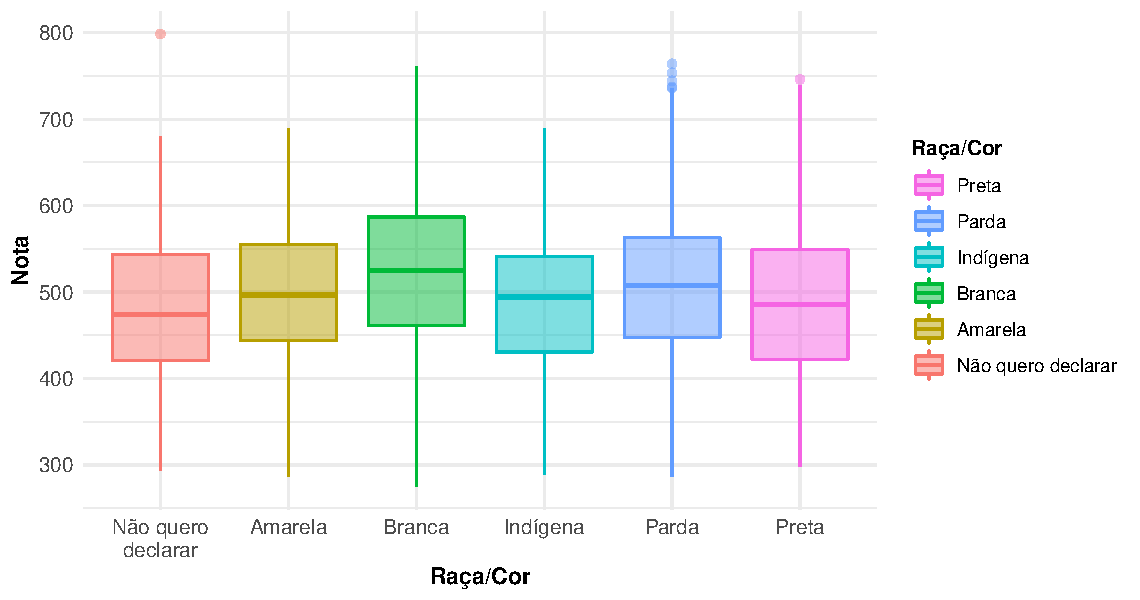
\includegraphics[width=16cm]{img/raca_cor_notas.pdf}
    \end{center}
    \fonte{Amostra de 5.271 alunos do 9\textsuperscript{o} ano do SAEB 2017.}
    \nota{Amostra retirada de uma amostragem aleatórias simples.}
\end{figure}
Sobre a \autoref{fig:raca_cor_notas}, nota-se que a soma das notas dos grupos tem uma
tendência da medida central (50\% dos alunos) ser localizada na nota 500, que varia pouco de 
acordo com a raça, sendo o fenótipo Branco aquele que possui as maiores valores nas medidas
de posição sobre as estas notas.

A raça Parda é a que possui o maior número de outliers entre os estudantes,
mas a maior nota observada esteve presente no grupo que não quis declarar a raça/cor.

\newpage
%%%% Grafico localizacao com notas

\begin{figure}[htb]
    \caption{Distribuições empíricas das somas das notas com base nas localizações das
    das escolas dos alunos.\label{img:loc_notas}}
    \begin{center}
        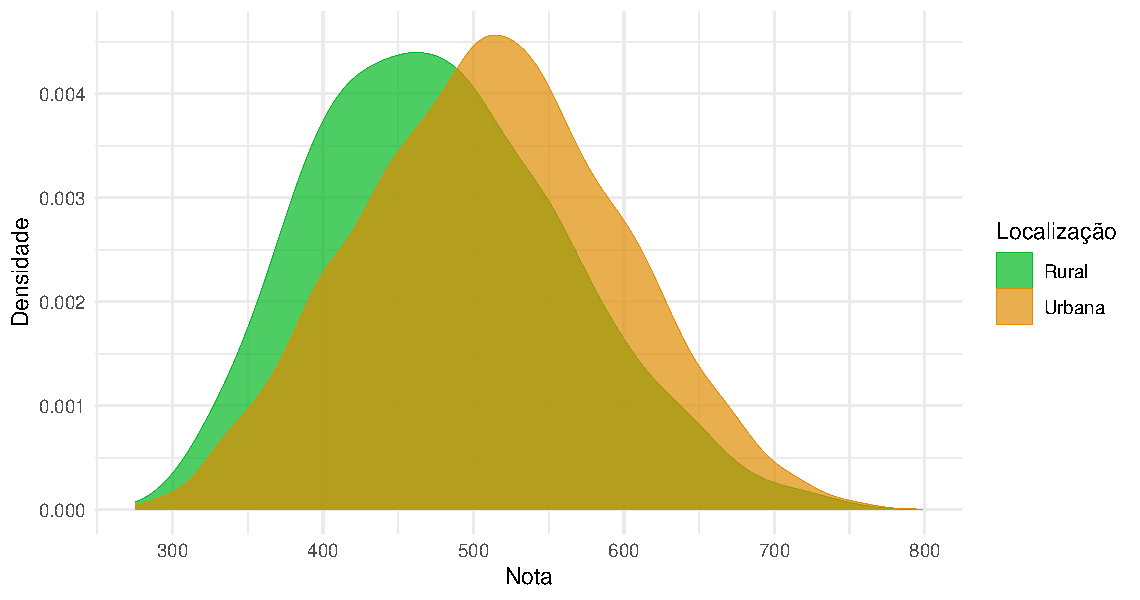
\includegraphics[width=16cm]{img/loc_notas.pdf}
    \end{center}
    \fonte{Amostra de 5.271 alunos do 9\textsuperscript{o} ano do SAEB 2017.}
    \nota{Amostra retirada de uma amostragem aleatórias simples.}
\end{figure}

Na \autoref{img:loc_notas}, é possível observar um grau de assimetria um pouco maior nestas notas para as escolas
das regiões rurais em relação às regiões urbanas. A distribuição das notas nas regiões rurais foi um pouco mais inclinada
para a esquerda e com moda inferior à moda das zonas urbanas, que possui uma distribuição mais centralizada.

As escolas rurais apresentaram uma nota média de 479, que também é inferior quando comparada com a nota média das
escolas urbanas, que foi de 512.

%%%%% Grafico da escolaridade da mae com notas

Para a \autoref{img:esc_mae_notas}, observa-se um crescimento das notas em geral, à medida que o grau de escolaridade
das mães é maior, de modo que apenas aqueles alunos que responderam que desconhecem a escolaridade da mãe
tiveram comportamento independente a essa observação. Esse comportamento é observado de forma equivalente aos valores extremos,
onde a maior nota registrada vem por parte do aluno cuja mãe completou a faculdade.
\newpage

\begin{figure}[h]
    \caption{Distribuições das somas das notas com base nas escolaridades 
    das mães dos alunos\label{img:esc_mae_notas}}
    \begin{center}
        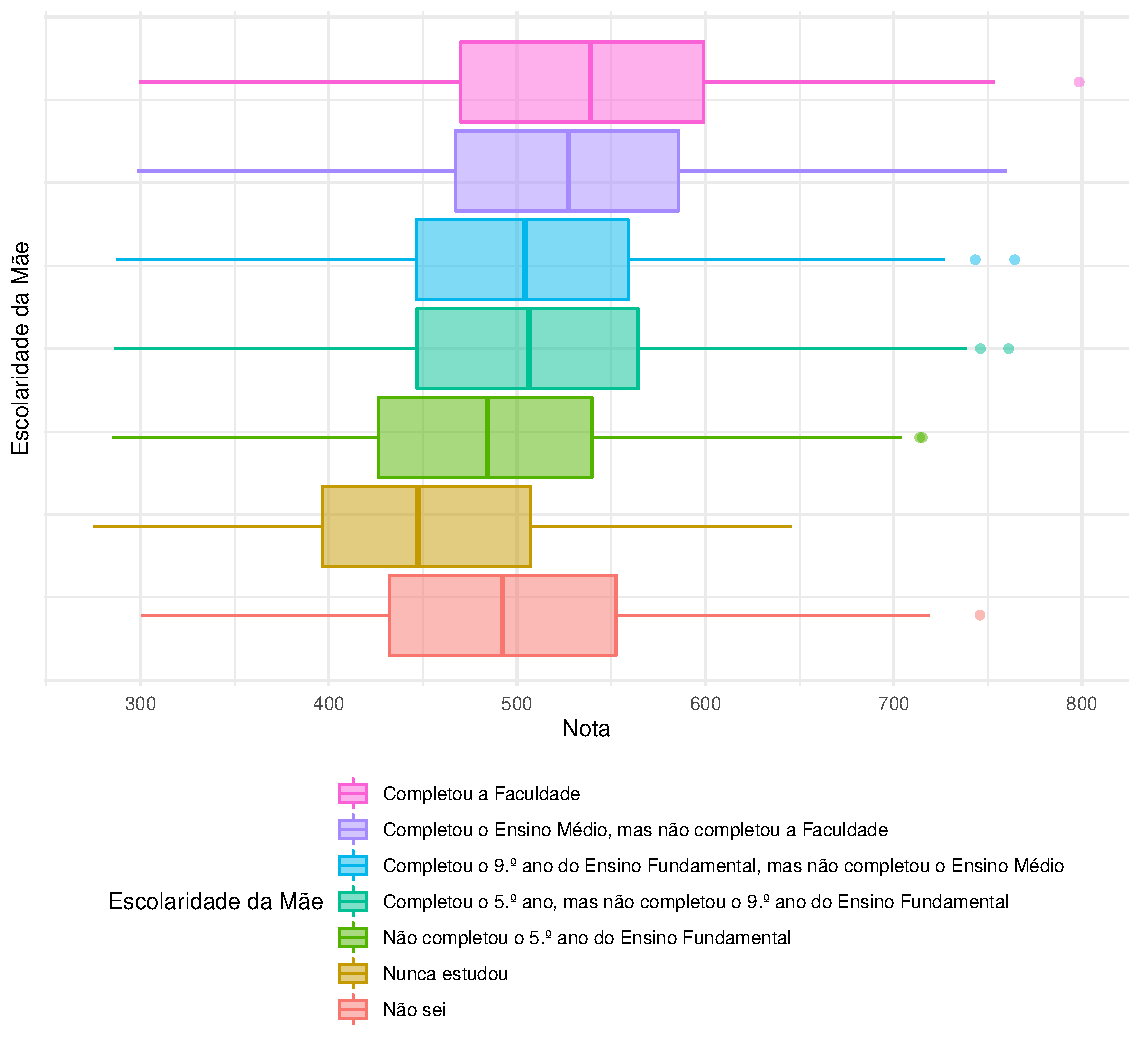
\includegraphics[width=16cm]{img/esc_mae_notas.pdf}
    \end{center}
    \fonte{Amostra de 5.271 alunos do 9\textsuperscript{o} ano do SAEB 2017.}
    \nota{Amostra retirada de uma amostragem aleatórias simples.}
\end{figure}





%%%%%%%%%%%%%%%%%%%%%%% Tabelas %%%%%%%%%%%%%%%%%%%%%%%%%%%%%%%%%%%%%%%%%%%%%%%%%%%%%%%%%%%%%%%%%
Ao realizar testes, verificou a hipótese das médias, desta soma de notas, se hávia indícios para aceitar
igualdades significativas com base nas relação efetuada pelo estudo, com a confiança 95\% para
aceitação estas hipóteses.
Para efetuar estes testes, foi avaliado primeiramente a hipótese de igualdade sobre as variâncias
das notas (Teste B) para cada relação abordada pelo estudo como as localizações das escolas, 
escolaridade da mãe, sexo e a raça/cor do aluno, no qual apenas a relação com o sexo rejeita esta hipótese
como demostra na \autoref{tab::tests_notas}.

\newpage
%%%%%% Tabela com testes para as relacoes das notas
\begin{table}[htb]
\caption{Testes para as relações com soma
 das notas dos alunos.\label{tab::tests_notas}}
    \centering
    \begin{tabular}{cccc}
    \toprule
    Teste & $H_0$& P-valor & Decisão de $H_0$ (95\%)\\
    \midrule \midrule
    B & $\sigma_R^2 = \sigma_U^2$ & 0.503 & Aceita\\
    B & $\sigma_M^2 = \sigma_F^2$ & 0.002 & Rejeita\\
    B & $\sigma_{Raça/Cor}^2$ iguais & 0.265 & Aceita\\
    B & $\sigma_{Esc(mãe)}^2$ iguais & 0.132 & Aceita\\
    T & $\mu_R = \mu_U$ & Aprox. 0 & Rejeita\\
    T & $\mu_M = \mu_F$ & 0.905 & Aceita\\
    ANOVA & $\mu_{Raça/Cor}$ iguais & Aprox. 0 & Rejeita\\
    ANOVA & $\mu_{Esc(mãe)}$ iguais & Aprox. 0 & Rejeita\\
    \bottomrule
    \end{tabular}
    \fonte{Amostra de 5.271 alunos do 9\textsuperscript{o} ano do SAEB 2017.}
    \nota{Amostra retirada de uma amostragem aleatória simples. Teste T dois a dois efetuado com a correção de 
    Bonferroni no P-valor.}
    \nota[Anotações]{Os subíndices, com base nos alunos, $R$ e $U$ refere-se as localizações
                    das escolas rurais e urbanas, M e F sobre os sexos Masculino e Feminino
                    respectivamente e Esc(mãe) diz respeito a escolaridade da mãe. 
                    O Aprox. 0 refere-se à algum número 
                    muito pequeno considerado por este estudo aproximadamente zero.}
\end{table}

% analise dos testes (tabela tab::tests_notas)
Ao concluir sobre estas relações com as variâncias na \autoref{tab::tests_notas}, foi avaliado estas
hipóteses de igualdades destas médias, que pelo mesmo nível de confiança, houve indícios de rejeita 
com base nos sexos (Teste T), que diz sobre não existir diferença em média entre estas notas com base no 
sexo do aluno. Sobe a mesma hipótese e as relações com a raça/cor do aluno e a escolaridade da mãe (Teste ANOVA)
sobre essas notas, houve indícios significativos de que em alguma destas relações houve alguma diferença 
com base na média, no qual testes dois a dois (Teste T) são apropriados para investigar qual foi estas diferenças.
Para a relação com as localizações das escolas, também foi rejeitada essa hipótese, no qual as escolas 
urbanas obteve em média, sobre esta soma de notas dos alunos, um valor superior que as escolas rurais.


\newpage
%%%%%% Tabela de comparacao entre raca/cor e notas

\begin{table}[htb]
    \centering
\caption{Comparações dois a dois entre as médias sobre a soma das notas
        com base na raça/cor dos alunos.\label{tab:raca_cor_notas}}
    \begin{tabular}{lcc}
    \toprule
    Comparações & P-valor & Evidência (RA 95\%)\\
    \midrule \midrule
    Amarela = Não quero declarar & 0.4113 & Iguais\\
    Amarela = Branca & 0.0005 & Desiguais\\
    Amarela = Indígena & 1.0000 & Iguais\\
    Amarela = Parda & 1.0000 & Iguais\\
    Amarela = Preta & 1.0000 & Iguais\\
    Branca = Não quero declarar & Aprox. 0 & Desiguais\\
    Branca = Indígena & 0.0010 & Desiguais\\
    Branca = Parda & Aprox. 0 & Desiguais\\
    Branca = Preta & Aprox. 0 & Desiguais\\
    Indígena = Não quero declarar & 1.0000 & Iguais\\
    Indígena = Parda & 0.7758 & Iguais\\
    Indígena = Preta & 1.0000  & Iguais\\
    Parda = Não quero declarar & Aprox. 0 & Desiguais\\
    Parda = Preta & Aprox. 0 & Desiguais\\
    \bottomrule
    \end{tabular}
    \centering
    \fonte{Amostra de 5.271 alunos do 9\textsuperscript{o} ano do SAEB 2017.}
    \nota{Amostra retirada de uma amostragem aleatória simples. Teste T dois a dois efetuado com a correção de 
    Bonferroni no P-valor.}
    \nota[Anotações]{Aprox. 0 refere-se à algum número muito pequeno considerando aproximadamente zero.}
    
\end{table}

Na \autoref{tab:raca_cor_notas}, as comparações dois a dois, apresentaram que a raça/cor branca obteve diferença,
nestes testes de hipótese de igualdade das médias, entre todas as outras raças, confirmando o que a 
\autoref{fig:raca_cor_notas} apontava.

As únicas desigualdades dessa hipótese, que não foram entre as comparações com os indivíduos da raça/cor branca,
foram entre as raças/cores dos alunos, pardos com os pretos e aqueles que não quiseram declarar.

Todos os outros testes não só levam à aceitação da hipótese de igualdade das médias ($H_0$), como apresentaram um p-valor
significativamente alto, que diz respeito à níveis de confiabilidades elevados.


%%%%% Tabela de comparação da notas com Escolaridade da mae
As hipóteses iniciais para a variável do nível de escolaridade da mãe, são passadas como comparações dois a dois na \autoref{tab:esc_mae_notas},
no que supõe esta hipóteses de igualdade entre as média, dessa soma das nota dos alunos, com cada grupo de nível escolar das mães.
\newpage

\begin{table}[htb]
    \centering
\caption{\label{tab:esc_mae_notas}Comparações dois a dois das notas entre os alunos com base na escolaridade da mãe}
    \begin{tabular}{lcc}
    \toprule
    Comparações & P-valor & Evidência (RA 95\%)\\
    \midrule \midrule
    Não sabe = Nunca estudou & Aprox. 0 & Desiguais\\
    Não sabe = Incompleto 5.\textsuperscript{o} ano do EF  & 1.0000 & Iguais\\
    Não sabe = Completou 5.\textsuperscript{o} ano do EF  & 0.0084 & Desiguais\\
    Não sabe = Completou 9.\textsuperscript{o} ano do EF  & 0.1927 & Iguais\\
    Não sabe = Completou EM & Aprox. 0 & Desiguais\\
    Não sabe = Completou Faculdade & Aprox. 0 & Desiguais\\
    Nunca estudou = Incompleto 5.\textsuperscript{o} ano do EF  & 0.0038 & Desiguais\\
    Nunca estudou = Completou 5.\textsuperscript{o} ano do EF  & Aprox. 0 & Desiguais\\
    Nunca estudou = Completou 9.\textsuperscript{o} ano do EF  & Aprox. 0 & Desiguais\\
    Nunca estudou = Completou EM & Aprox. 0 & Desiguais\\
    Nunca estudou = Completou Faculdade & Aprox. 0 & Desiguais\\
    Incompleto 5.\textsuperscript{o} ano do EF = Completou 5.\textsuperscript{o} ano do EF  & 0.0002 & Desiguais\\
    Incompleto 5.\textsuperscript{o} ano do EF = Completou 9.\textsuperscript{o} ano do EF  & 0.0048 & Desiguais\\
    Incompleto 5.\textsuperscript{o} ano do EF = Completou EM & Aprox. 0 & Desiguais\\
    Incompleto 5.\textsuperscript{o} ano do EF = Completou Faculdade & Aprox. 0 & Desiguais\\
    Completo 5.\textsuperscript{o} ano do EF = Completou 9.\textsuperscript{o} ano do EF  & 1.0000 & Iguais\\
    Completo 5.\textsuperscript{o} ano do EF = Completou EM & Aprox. 0 & Desiguais\\
    Completo 5.\textsuperscript{o} ano do EF = Completou Faculdade & Aprox. 0 & Desiguais\\
    Completo 9.\textsuperscript{o} ano do EF = Completou EM & Aprox. 0 & Desiguais\\
    Completo 9.\textsuperscript{o} ano do EF = Completou Faculdade & Aprox. 0 & Desiguais\\
    Completou EM = Completou Faculdade & 1.0000 & Iguais\\
    \bottomrule
    \end{tabular}
    \centering
    \fonte{Amostra de 5.271 alunos do 9\textsuperscript{o} ano do SAEB 2017.}
    \nota{Amostra retirada de uma amostragem aleatória simples. Teste T dois a dois efetuado com a correção de 
    Bonferroni no P-valor.}
    \nota[Anotações]{Aprox. 0 refere-se à algum número muito pequeno considerando aproximadamente zero e 
    EF e EM remete ao ensino fundamental e ensino médio respectivamente.}
    
  \end{table}

E dentre esses grupos, somente os grupos que aqueles alunos que declararam não saber a escolaridade da mãe com aquelas mães que tem o
5\textsuperscript{o} incompleto ou 9\textsuperscript{o} completo, aquelas mães que tem completo o 5\textsuperscript{o} com as que tem
9\textsuperscript{o}, com base no ensino fundamental, e aquelas que tem completo o ensino médio com as que as que possui a 
faculdade completa, esta hipótese foi rejeitada, com um nível de significância de 95\%. Ao considerar estas igualdades e 
as outras desigualdades das médias sobre a soma destas notas, há maiores valores para aquelas mães que possuem
níveis de escolaridade superiores.